% Implementação do projecto
\chapter{Validação}
\label{cap5}

\section{Testes com utilizadores}

Para testar a facilidade de utilização do dispositivo e a responsividade do nosso protótipo realizamos testes com alguns utilizadores reais. No entanto é de realçar que estes utilizadores não correspondem exactamente à caracterização de utente que escrevemos anteriormente. Esta escolha deveu-se ao facto de estes serem testes muito iniciais que visam apenas verificar o funcionamento básico do aparelho, detectar problemas relacionados com a implementação do mesmo e tentar obter um feedback básico em relação ao mesmo.
Deste modo pedimos aos 5 utilizadores que fizessem três testes simples:
\begin{itemize}
	\item Simular uma ocorrência em que o utente acciona-se o botão de SOS;
	\item Simular uma ocorrência em que o utente sofre-se uma queda;
	\item Simular uma ocorrência em que o utente se mantivesse imóvel durante um período de tempo de 2 minutos;
\end{itemize}

A figura \ref{fig:testes}, mostra o conjunto de utilizadores a efectuarem os testes. É de referir que com o propósito de agilizar os testes diminuímos o tempo de imobilidade para 2 minutos.
No final dos testes realizamos, a cada um dos utilizadores um questionário oral sobre a utilização do dispositivo, e perguntamos se desejavam mencionar alguma critica ou melhoria que pudesse-mos ter em consideração.

\begin{figure}[!htb]
	\centering
	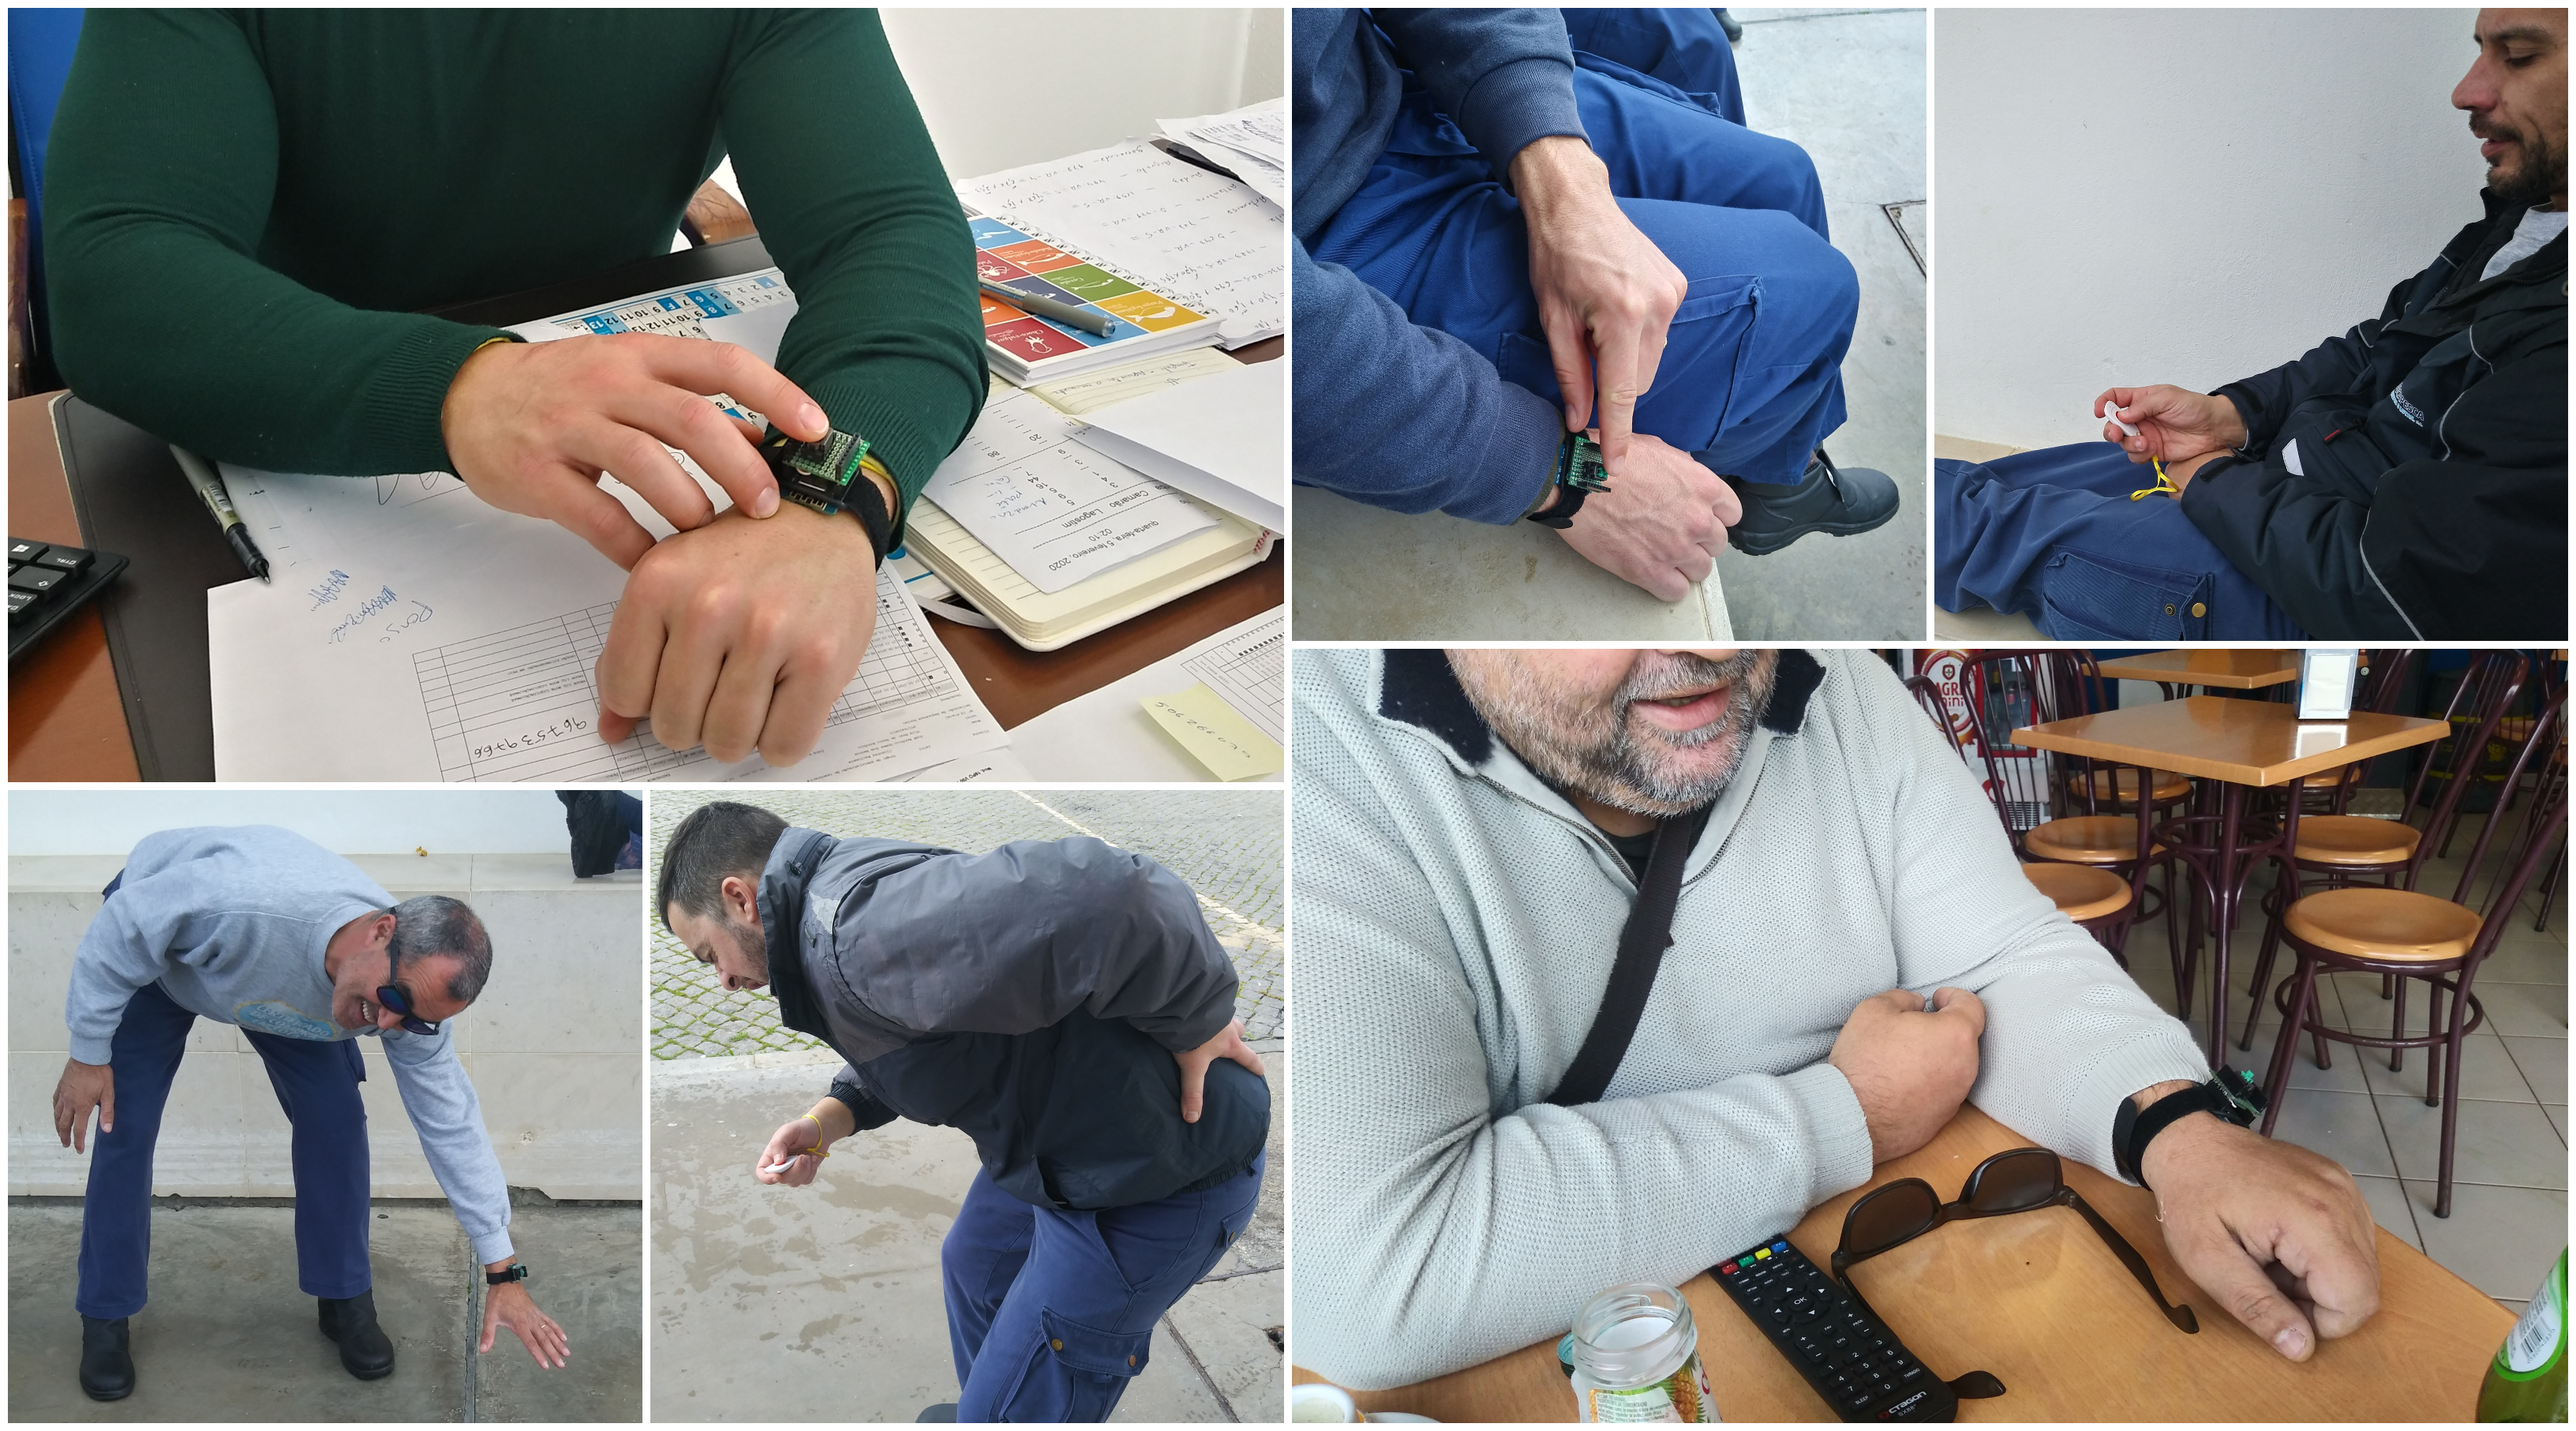
\includegraphics[width=1.0\textwidth]{figuras/testes.png}
	\caption{Testes com utilizadores}
	\label{fig:testes}
\end{figure}

%\subsection{Planeamento dos testes}

%\subsubsection{Objectivos dos testes}
%\subsubsection{Que participantes serão recrutados}A
%\subsubsection{Que métricas de desempenho e de satisfação serão usadas para recolher dados	da experiência?}B
%\subsubsection{Escrita de tarefas a propor ao utilizador e definição de como lhe serão	comunicadas}C
%\subsubsection{Quem conduz os testes? Quem interpreta o “Computador-Humano”? Quem mais participa nos testes?}D
%\subsubsection{Onde, quando duração, material/equipamento, e que outros recursos serão necessários definir?}E
%\subsubsection{Como será apresentado o protótipo:}
%\subsubsection{Comportamento a pedir aos utilizadores}
%\subsubsection{Métodos de registo}
%\subsubsection{Qual é o Protocolo da experiência}
%\subsubsection{Ajuda e documentação}

%\subsection{Execução dos testes}

\FloatBarrier\subsection{Resultados dos testes}

Todos os testes realizados pelos utilizadores produziram os avisos esperados no portal, os quais foram encaminhados para o e-mail do piquete que preparamos para o efeito. Os tempos de envio foram sempre inferiores a 1 minuto, tal como desejado.

\subsection{Propostas de redesenho}

Os utilizadores referiram algumas criticas, as quais passamos a enumerar:
\begin{itemize}
	\item O corpo do dispositivo é demasiado volumoso, tornando-se pouco prático transportar o mesmo;
	\item O botão de SOS não transmite a sensação de ter sido pressionado;
	\item O dispositivo não inclui um aviso sonoro que indique uma ocorrência;
\end{itemize}

Os utilizadores não mencionaram nenhuma melhoria.

\section{Trabalho futuro}



\section{Conclusão}

 